\chapter{Theoretische Grundlagen}

In diesem Kapitel werden die für den Forschungshintergrund und für die Entwicklung des Prototyps wichtigen theoretischen Grundlagen vorgestellt.
Zunächst werden verschiedene Theorien zu Kommunikationsmodellen vorgestellt, auf deren Basis das Modell für diese Anwendung zugrunde liegt.
Im Anschluss daran werden die in der Ludologie beschriebenen Akteure vorgestellt, welche sich in den Probanden dieser Masterarbeitsstudie wiederfinden werden. Allgemein ist bekannt, dass Video- und Computerspiele drei verschiedene Modi haben können: Singleplayer, Multiplayer und Mischformen. Da für den Zweck dieser Studie ein Multiplayer-Spiel konzipiert und umgesetzt wurde, werden im weiteren Verlauf verschiedene Kategorien von Multiplayer-Spielen vorgestellt. Außerdem werden die damit einhergehenden Netzwerkinfrastrukturen vorgestellt, die relevant sind und für die weitere Entwicklung relevant sein könnten.

\section{Kommunikationsmodelle}
[Literatur suchen]
% In der Kommunikationswissenschaft wird die Kommunikation in 2 Arten unterteilt, die Massen- und Individualkommunikation.

\subsection{Nach Schulz von Thun}
\subsection{Nach Wazlawik}
\subsection{Nach Rogers}

% [Könnte besser in die Einleitung passen
% \section{Spiele als soziales Medium}
% \cite{depping_trust_2016}
% \cite{gerling_designing_2014}
% \cite{ducheneaut_alone_2006}
% ]

\section{Spielertypen}
Die Kommunikationswissenschaft umfasst zwar den Hauptteil dieser Arbeit, allerdings beinhaltet diese ebenfalls ludologische Aspekte. Dabei geht es um die Lehre über das Spiel (vgl. \cite{ludologie_spielforschung_nodate}). 

Im Hinblick auf die Konzeption und die Entwicklung eines Spiels ist es wichtig, die Eigenschaften des Spielsystems so zu gestalten, dass sich Begeisterung und Engagement bei der gewünschten Zielgruppe hervorrufen. Aus diesem Grund muss zunächst die Zielgruppe in verschiedene Typen eingeteilt werden. In der Ludologie gibt es dafür verschiedene Spielertypen. Zwar ist nicht jeder Mensch ein \say{Spielertyp}, grundsätzlich kann er jedoch über verschiedene Spielelemente angesprochen werden (vgl. \cite{ludologie_spielertypen_nodate}).

\subsection{Nach Bartle}
1996 beschäftigte sich Richard Bartle mit der Frage, welche Spielertypen es in der Ludologie gibt. Dabei ging es zunächst um die Klassifizierungen, welche Ansätze es beim Spielen von sogenannten \ac{MUD}s existieren (vgl. \cite{bartle_hearts_1996}). Diese Klassifizierungen werden noch heute für die Einteilung in Spielertypen genutzt.

Bartle unterscheidet bei der Einteilung der Spielertypen auf zwei unterschiedliche Grundinteressen (vgl. Abbildung \ref{fig:bartle-muds}):

\begin{figure}[ht]
\centering
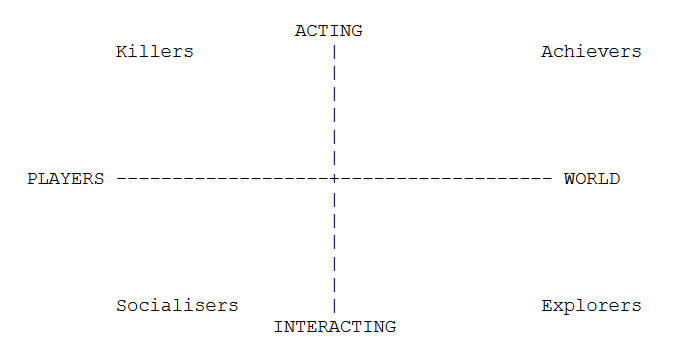
\includegraphics[width=1\linewidth]{content/pictures/basic_interests.PNG}
\caption{Interessen Graph nach Bartle (vgl. \cite{bartle_hearts_1996})}
\label{fig:bartle-muds}
\end{figure}

In X-Achsen-Richtung wird unterschieden, ob der Spieler seine Spielerfahrung über das Verhalten der anderen Mitspieler (Players) oder der Spielwelt (World) bevorzugt. Auf der Y-Achsen-Richtung unterscheidet er, ob der Spieler bevorzugt, selbst einen Einfluss auf die Spielwelt zu geben und diese beeinflusst (Acting) oder ob er in tiefere Interaktion mit der Spielwelt eingehen will (Interacting).

Die daraus resultierenden Typen sind:
\paragraph{Achiever}
Sie sind daran interessiert, auf die Welt einzuwirken, um dadurch in sie eintauchen zu können. Sie wollen das Spiel meistern und dazu bringen, das zu tun, was sie wollen. Ihr Status im Spiel ist ihnen wichtig und die wenige Zeit, die sie dafür benötigt haben.

\paragraph{Explorer}
Sie wollen vom Spiel überrascht werden und mit der Spielwelt interagieren. Die virtuelle Welt löst ein Gefühl des Staunens aus, nach dem sie sich sehnen. Sie sind stolz auf das Wissen über das Spiel, das sie sammeln, und wollen dieses Wissen gerne an neue Spieler weitergeben.

\paragraph{Socialiser}
Sie wollen mit anderen Spielern interagieren. Zumeist erfolgt das über Gespräche, es kann aber auch ungewöhnliche Verhaltensweisen einschließen. Andere Menschen kennenzulernen und mehr über sie zu erfahren, ist für sie wertvoller als für andere. Die Spielwelt ist für sie nur eine Kulisse, für sie sind andere Charaktere fesselnder. Sie sind stolz auf Freundschaften, ihre Kontakte und ihren Einfluss.

\paragraph{Killer}
Sie sind daran interessiert, auf andere Spiele einzuwirken und mit ihnen Dinge zu machen. Im Allgemeinen erfolgt dies ohne das Einverständnis der anderen Spieler. Sie wollen ihre Überlegenheit gegenüber anderen Menschen demonstrieren. Sie sind stolz auf ihren Ruf und oft geübten Kampffähigkeiten.

(vgl. \cite{bartle_hearts_1996}).

\subsection{Erweiterte Einteilungen}
Bartle ist nicht der Einzige, der sich mit Spielertypen auseinandergesetzt hat. Seine Forschung gilt als Fundament, welches in der weiteren Forschung für Diskussionen in der Forschungs- und Game-Design-Community gesorgt hat. 
\begin{quote}
    \textit{
        \enquote{Player types are not a defined concept and any categorization of players or users needs to occur within the context of a particular application or domain. Play-personas are suggested as a useful tool that can be used to put player type research into practice as part of the design process of gamified systems.}
    } 
    (\cite{dixon_player_nodate})
\end{quote}

\paragraph{Dixon} 
stellt Spieler-Personae vor, die wie im \ac{UCD}-Prozess verwendet werden können. Dadurch muss im Designprozess nicht zu sehr zwischen Motivation, Verhalten oder Vorlieben unterschieden werden, da Personae als reichhaltige und erzählerische Darstellung gedacht sind (vgl. \cite{dixon_player_nodate}).

\paragraph{Bateman und Boon}
benutzen in ihrer 2005 erschienen Studie zur Bestimmung des ersten Modells des demografischen Game Designs (DGD1) vier Spielstile, welche sie durch die Hinzunahme der Myers-Briggs Type Indicator (vgl. \cite{noauthor_mbti_nodate}) ableiteten (vgl. \cite{bateman_21st_2005}).
Conquerer (Eroberer), Manager, Wanderer (Wanderer) und Participant (Teilnehmer) waren dabei die vier Spielstile.

In einer zweiten Studie wurden vier hypothetische Spielstile erstellt, welche von einer Studie von Berens 2000 (vgl. \cite{berens_understanding_2000}) abgeleitet wurden (vgl. \cite{bateman_player_2012}). Die resultierenden Stile sind folgende: Logistical, Tactical, Strategic und Diplomatic.

Im Kern sind diese Modelle Ableitungen von Bartles ursprünglicher Metrik (vgl. \cite{ludologie_spielertypen_nodate}).

\paragraph{Yee}
Nick Yee entwickelte empirisch fundiertes Modell zur Beschreibung von Spielmotivationen in Online-Spielen, das bis heute einen großen Einfluss auf die Ludologie hat. Mittels eines faktorenanalytischen Ansatzes untersuchte er eine Vielzahl an Daten aus Online-Umfragen und identifizierte dabei 10 spezifische Motivationsgruppen, die in drei übergeordnete Hauptkategorien gegliedert werden (vgl. Abbildung \ref{fig:nick_yee_motivations}):

\begin{figure}[ht]
\centering
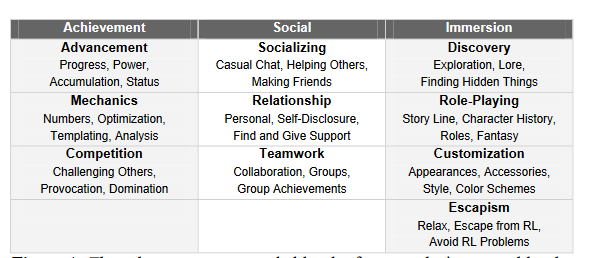
\includegraphics[width=1\linewidth]{content/pictures/nick_yee_categorizations.PNG}
\caption{Motivationsgruppen nach Nick Yee (vgl. \cite{yee_motivations_nodate})}
\label{fig:nick_yee_motivations}
\end{figure}

Die Achievement-Komponente umfasst den Fortschritt im Spiel, sowie das damit einhergehende Verlangen Macht zu erlangen, schnell voranzukommen und Symbole von Reichtum oder Status im Spiel zu erlangen. Außerdem existiert ein Interesse daran, die Mechanik des Spiels zu analysieren, die Regeln und Systeme zu verstehen um die Leistung der Spielfigur zu optimieren. Außerdem ist der Wettbewerb wichtig. Es besteht der Wunsch danach sich mit anderen zu messen und gegen sie anzutreten.

Die soziale Komponente beschreibt dabei die Sozialisierung der Spieler, bei denen sie Interesse daran haben anderen Spielern zu helfen und sich mit ihnen zu Unterhalten. Daraus entstehen Beziehungen, bei denen der Wunsch nahe liegt, dass langfristige und bedeutungsvolle Beziehungen zu anderen aufgebaut werden können. Außerdem ist Teamarbeit gewünscht, um sich gegen andere zu messen und gegen sie anzutreten.

Die Immersions-Komponnete beschreibt das Entdecken in der Spielwelt und dem damit einhergehende finden von Dingen, Wissen zu erlangen, welches den meisten anderen Spielern unbekannt ist. Rollenspiel-Elemente sind dabei besonders wichtig, um den Spielfiguren eine Hintergrundgeschichte zu geben und gemeinsam eine improvisierte Geschichte zu entwickeln. Der Spielavatar sollte auch anpassbar sein, damit der individuelle Geschmack der Spieler in das Spiel einfließen kann. Die Spiel-Welt wird genutzt um von den Problemen der realen-Welt zu entkommen.

\paragraph{weitere Modelle}
Im Zuge der fortschreitenden Forschungen entstanden weitere Modelle wie das Gamer Motivation Model, das auf Basis der Forschung von Nick Yee entwicjelt wurde (vgl. \cite{ludologie_spielertypen_nodate}):

\begin{figure}[ht]
\centering
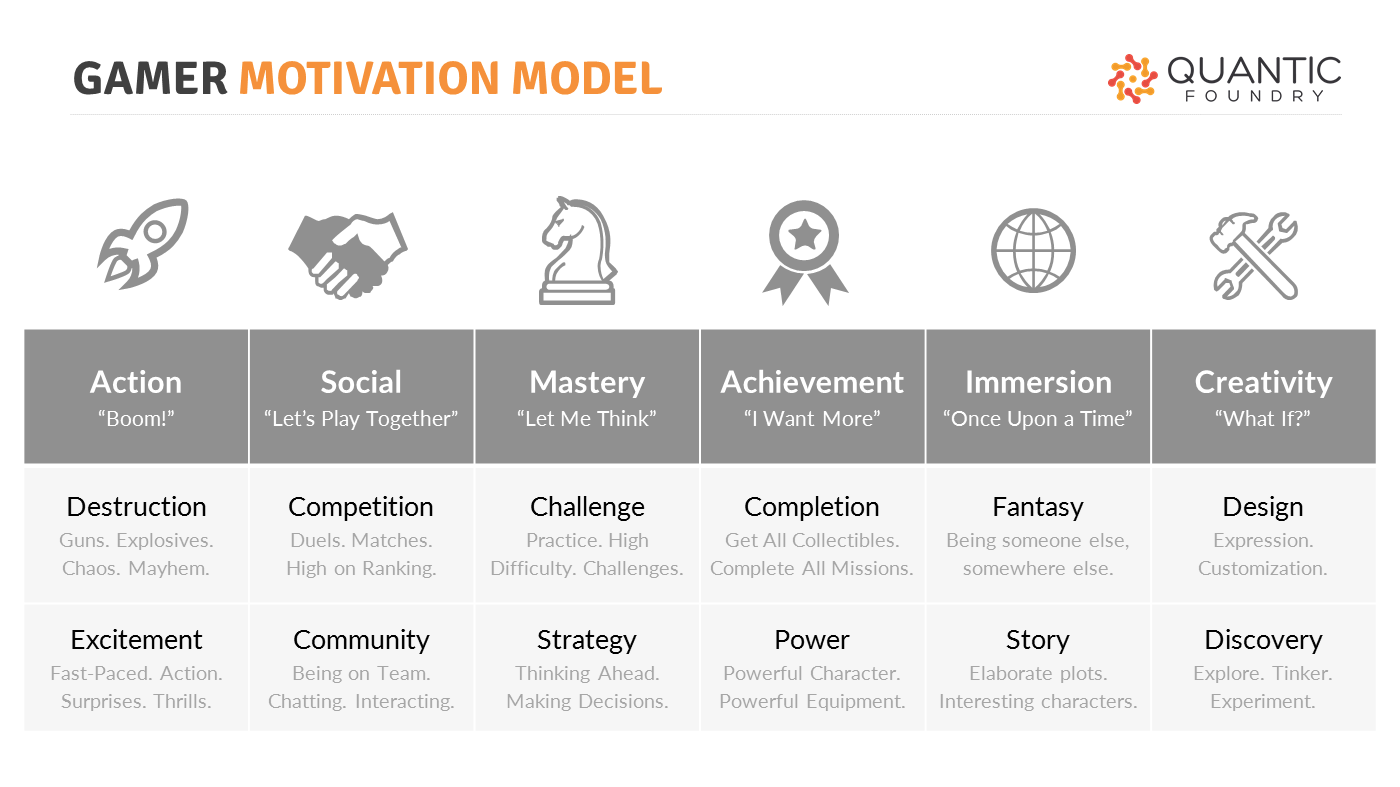
\includegraphics[width=1\linewidth]{content/pictures/gamer_motivations_model.png}
\caption{Gamer Motivation Model der QUANTIC FOUNDRY (vgl. \cite{noauthor_quantic_nodate})}
\label{fig:gamer_motivation_model}
\end{figure}

Ein weiteres Modell, das in der Arbeit von Bateman genannt wird, ist das BRAINHEX-Model, bei dem die verschiedenen Spielertypen in Hexagonaler Anordnung platziert werden (vgl. Abbildung: \ref{fig:brain-hex}):

\begin{figure}[ht]
\centering
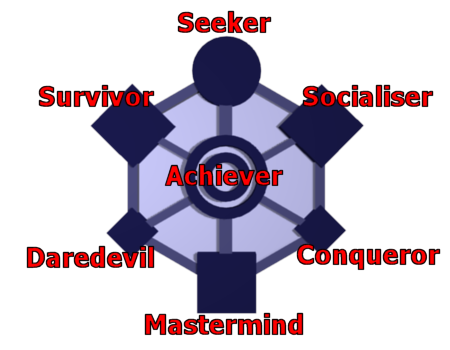
\includegraphics[width=1\linewidth]{content/pictures/brainhex-classes.png}
\caption{Brainhex-Model Darstellung von \cite{noauthor_i_nodate} nach \cite{nacke_brainhex_2013}}
\label{fig:brain-hex}
\end{figure}

% \cite{bartle_hearts_nodate}

% [erwähnen wurde aber rausgelassen, man kann erwähnen, dass es noch weitere klassifizierungen gibt
% \subsection{Das BrainHex-Model}
% \cite{nacke_brainhex_2014}
% ]

% [kommt zu wichtige Begriffe
% \section{Kooperative Gamedesign Pattern}
% \subsection{Was sind Game Pattern}
% \cite{bjork_patterns_2005}

% \subsection{Complementarity}

% \subsection{Synergies}

% \subsection{Abilities}

% \subsection{Shared Goals}

% \subsection{Synergies between goals}

% \subsection{Special Rules for Player of the same Team}

% \subsection{Camera Setting}

% \subsection{Interacting with the same object}

% \subsection{Shared puzzle}

% \subsection{Shared characters}

% \subsection{Special characters targetting lone wolf}

% \subsection{Vocalization}

% \subsection{Limited ressources}

% \subsection{Einflussnahme}
% \cite{emmerich_impact_2017}

% ]
\section{Multiplayer-Spiele}
Im Vergleich zu Einzelspieler-Spielen existieren bei Multiplayer-Spielen nicht nur Unterscheidungen im Genre des Spiels, sondern auch in den Spielrollen (Symmetrie / Asymmetrie) sondern auch in den Spielzeitpunkten (Synchron / Asynchron) wann die Spielteilnehmer an ihrem Sportfortschritt weiter arbeiten. [Hier wäre eine Quelle noch gut]. Auf dem Spielemarkt existieren außerdem Multiplayer-Spiele, die unterschiedliche Medientechniken verwenden. Teilweise werden diese Medientechniken verwendet um eine Cross-Plattform Funktionalität zu gewährleisten (vgl. \cite{noauthor_baldurs_nodate}) oder es ist Teil des Gamedesigns (vgl. \cite{noauthor_keep_nodate}}).

Da im Kontext von \say{Connecting-Minds} die Spieler zeitgleich in einer Sitzung gemeinsam spielen, wird im folgenden auf die symmetrie / asymmetrie von Computer- und Videospielen eingegangen.

% In den folgenden Kapiteln werden die jeweiligen Eigenschaften der unterschiedlichen Ausprägungen von Multiplayer-Spielen aufgezählt.

% \subsection{Synchrone Multiplayer}
% Synchrone Multiplayer-Spiele sind solche, bei denen die Spieler i. d. R. zum selben Zeitpunkt, bzw. zur selben Zeit gemeinsam miteinander oder gegeneinander Spielen. [Quelle suchen]. Weit verbreitet sind hier vorallem Ego-Shooter wie die \say{Call of Duty}-Reihe, bei denen die Spieler innerhalb einer Sitzung gegeneinander im \say{Einzel} oder als \say{Team} gegeneinander Spielen (vgl. \cite{noauthor_call_nodate}).

% \subsection{Asynchrone Multiplayer}
% Asynchrone Multiplayer-Spiele werden zeitversetzt gespielt. [Quelle und beispiele suchen]

\subsection{Symmetrische Multiplayer}
Symmetrische Spiele sind die, bei denen alle Spieler die selben Spielregeln haben und das gleiche Spielziel verfolgen. Viele traditionelle Spiele wie Schach oder Computer- und Videospiele wie \say{Mario Kart} oder \say{Minecraft} sind symmetrische Multiplayer-Spiele, bei denen für jeden Spieler das gleiche Ziel gilt (vgl. \cite[S. 12]{adams_fundamentals_2013}), (vgl. \cite{noauthor_mario_nodate}), (vgl. \cite{noauthor_willkommen_nodate}). 


\subsection{Asymmetrische Multiplayer}
Asymmetrische Spiele hingegen können unterschiedliche Spieler unterschiedliche Regeln haben und versuchen ebenfalls unterschiedliche Ziele zu erreichen (vgl. \cite[S. 12]{adams_fundamentals_2013}). Sie sind in kooperativen und kompetitiven Spielen weit verbreitet und sind bspw. in Form von verschiedenen \say{Helden} oder \say{Klassen} umgesetzt. So gibt es z.B. in \say{Overwatch} oder \say{League of Legends}  unterschiedliche \say{Support}-Charaktere, deren Aufgabe es ist das Team zu heilen (vgl. \cite{smilovitch_birdquestvr_2019}), (vgl. \cite{noauthor_league_2025}), (vgl. \cite{noauthor_overwatch_nodate}). 
Außerdem ermöglichen sie, dass Spieler mit unterschiedlichen Fähigkeiten und Fähigkeitsniveaus gemeinsam spielen können. Ein asymmetrisches Design kann zudem die Inklusivität in Spielen fördern (vgl. \cite{smilovitch_birdquestvr_2019}).

\subsection{Hybride Multiplayer}
Wie \cite[S. 6f]{lotz_konzeption_2021} in ihrer Bachelor-Arbeit beschrieben hat, unterscheiden sich Multiplayer auch in ihrer genutzten Medientechnik. Sogenannte hybride Spiele wie \say{New Super Mario Bros U} (vgl. \cite{noauthor_mario_nodate-1}).

\begin{figure}[ht]
\centering
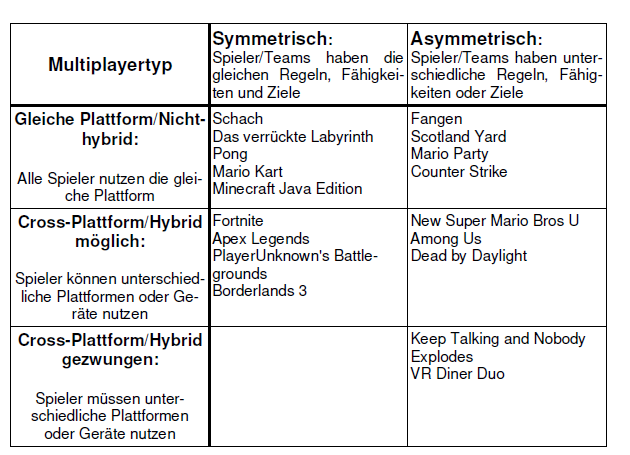
\includegraphics[width=1\linewidth]{content/pictures/lotz_hybrid_multiplayer.PNG}
\caption{Unterscheidung Multiplayertypen nach \cite[S.6]{lotz_konzeption_2021}}
\label{fig:lotz_multiplayer_types}
\end{figure}

Wie Abbildung \ref{fig:lotz_multiplayer_types} zeigt, können Multiplayer-Spiele, auf ihre Medientechnik bezogen, in 3 Kategorien eingeteilt werden.
Spiele wie \say{Mario Kart} oder \say{Minecraft} können nur über die gleiche Plattform gespielt werden. Bei Spielen wie \say{Among Us} oder \say{Fortnite} ist die Plattform, über die gespielt wird, nicht wichtig, da eine Cross-Play-Funktionalität gegeben ist. Jeder kann mit Spielern auf der Plattform spielen, die er bei sich zuhause hat. Die Kategorie ist die, bei der die Spieler gezwungen werden, unterschiedliche Plattformen zu nutzen. In \say{Keep talking and nobody explodes} ist das der Kern des Gamedesigns.

\section{Spielweisen von Multiplayer-Spielen}
Nachdem die unterschiedlichen Strukturen und technischen Formen von Multiplayer-Spielen behandelt wurden, ist es nun wichtig, darauf zu schauen, welche unterschiedlichen Spielweisen sie haben können. Multiplayer-Spiele können dabei in 3 unterschiedliche Spielformen unterschieden werden:
auf competitive, collaborative und cooperative Spielweisen. [Quelle finden]

\subsection{Kompetetiv}
Kompetitive Spiele sind Spiele, bei denen Kombinationen von verschiedenen Spielern gewinnen müssen, während eine andere Kombination von Spielern verlieren oder gemeinsam gewinnen muss. Das Spiel selbst kann weder verlieren noch gewinnen (vgl. \cite{noauthor_game_2014}). [noch andere Quellen suchen]

\subsection{Kollaborativ}
Kollaborative Spiele sind solche, bei denen alle Spieler wie in einem Kooperationsspiel gemeinsam gegen das Spiel verlieren können. Alle zusammen können aber nicht gewinnen. Diese Spiele sind im Kern meist kompetitiv, beinhalten aber die Möglichkeit einer kollektiven Niederlage. Die Spieler müssen zu einem gewissen Maße zusammenarbeiten um nicht zu verlieren (vgl. \cite{noauthor_game_2014}). [noch andere Quellen suchen]

\subsection{Kooperativ}
Bei Kooperationsspielen ist es möglich, dass alle Spieler gemeinsam gegen das Spiel verlieren oder gewinnen können. Ein Sieg wird erreicht, wenn das Spiel gemeinsam \say{besiegt} wird, oder dadurch dass ein festgelegtes Ziel gemeinsam oder individuell erreicht werden konnte (vgl. \cite{noauthor_game_2014}). [noch andere Quellen suchen]

\section{Artverwandte Spiele}
% Hier kommen die analysierten Spiele rein, also die Auflistung der Spiele, die ich mir im Zuge angesehen habe
Nachdem nun die einzelnen Charakteristiken von Multiplayer-Spielen aufgezeigt wurden, werden nun Spiele vorgestellt, welche im Rahmen dieser Arbeit näher betrachtet wurden.

Die Spielreihe \say{\textbf{We were here}} vom niederländischen Entwicklerstudio Total Mayhem Games beinhaltet asymmetrische Kooperative-Multiplayer-Spiele, bei denen zu zweit Rätsel und Hindernisse in der Spielwelt gelöst werden müssen um aus der Umgebung, in denen die Avatare der Spieler gefangen sind, zu entkommen. Dabei können die Spieler über ein \say{In-Game}-Walki-Talki miteinander kommunizieren. Zumeist ist es so, dass ein Spieler verschiedene Rätsel oder Hindernisse für sich hat, die er seinem Mitspieler beschreiben muss, damit dieser die passenden Antworten übermitteln oder Rätsel lösen kann. Die beiden Spieler befinden sich dabei in abgetrennten Räumen oder Gebieten innerhalb der Spielwelt (vgl. \cite{noauthor_we_nodate}; \cite{noauthor_total_nodate}).  

Das Spiel \say{\textbf{The past within}} vom ebenfalls aus den Niederlanden kommenden Entwicklerstudio Rusty Lake ist ein asymmetrisches kooperatives Multiplayer-Spiel bei dem zwei Spieler gemeinsam in einer Sitzung sowohl in der Vergangenheit als auch in der Zukunft gemeinsam Rätsel lösen müssen um der Protagonistin und ihrem Vater zu helfen. Jeweils ein Spieler befindet sich dabei in einer 2D-Amnwendung, der andere in einer 3D-Anwendung. Es existiert die Möglichkeit, dass das Spiel von verschiedenen Plattformen aus gespielt werden kann (Cross-Plattform Spielbarkeit) (vgl. \cite{noauthor_past_nodate}). 

Das bereits in den vorangegangenen Kapiteln [Kapitel einbinden] erwähnte \say{\textbf{Keep Talking and Nobody Explodes}} ist ein asymmetrisches kooperatives Multiplayer-Spiel bei dem eine Person das Spiel besitzen muss damit es im Team gespielt werden kann. Das Spiel hat eine Besonderheit, da es ein Cross-Plattform Spiel ist, bei dem ein Teilnehmer (der Bombenentschärfer) eine Bombe entschärfen muss und die anderen Spielteilnehmer (die Experten) verschiedene Anleitungen von Bomben vorliegen haben. Die Aufgabe besteht darin die richtige Anleitung für die entsprechende Bombe zu finden und die Bombe innerhalb der vorgegebenen Zeit zu entschärfen. Im Spiel befindet sich jedoch nur der Bombenentschärfer, während die Experten die Anleitungen ausgedruckt durchschauen können (vgl. \cite{noauthor_keep_nodate}).

Im März 2025 erschien das Spiel \say{\textbf{Myrmidon}} vom Studio Studio Popot, welches ein asymmetrischer kooperativer Multiplayer ist, bei dem zwei Spieler zusammen, in zwei verschiedenen Rollen, miteinander spielen können. Eine Rolle ist dabei die Stop-Motion Puppe, welche in einer Stop-Motion Welt Hindernisse überqueren und über verschiedene Plattformen springen muss um ans Ziel zu kommen. Unterstützt wird die Puppe dabei vom Animator, der die Kulisse des Stop-Motion Films bedienen muss, damit die Puppe an ihr Ziel gelangt (vgl. \cite{noauthor_myrmidon_2024}).

\section{Netzwerkinfrastrukturen}

enthält eine Liste von Möglichkeiten, auf welcher Grundlage verschiedene Multiplayer-Anwendungen gebaut werden können


\chapter{Verwandte Arbeiten}

\cite{harris_asymmetry_2019}
\cite{sajjadi_maze_2014}

hier würden Paper reinkommen die asymmetrische Multiplayer gemacht haben, welche aspekte da mitreinspielen, da kommen dann auch die wichtigen Begriffe dazu mitrein. Auch bereits umgesetzt asymetrische VR Spiele?


Auch Anna Lotz´ Thesis wäre hier relevant


\section{Wichtige Begriffe}

\subsection{Interdependence}
\cite{harris_leveraging_2016}
\cite{depping_cooperation_2017}

\subsection{Degrees of Interdependence}
\cite{beznosyk_effect_2012}

\subsection{Soziale Präsenz}

Vertrauen gibts in dem Kontext auch und wie man dan über Spiele aufbaut

\section{Untersuchungsschwerpunkte}